\chapter{Dynamic strip load on 2D elastic halfspace}


% ----------------------------------------------------------------------------------------------
\section{Introduction}
% ----------------------------------------------------------------------------------------------
This benchmark compares the STEM numerical solution against the analytical solution,
where a dynamic line load is applied along the surface of an elastic half-space discretised in a plane-strain setting.

The analytical solution is presented in~\cite{Verruijt_Brinkgreve_Li_2008}.
The analytical solution provides closed-form expressions for the vertical stress along the surface of the
half-space, enabling a direct time-history comparison against the numerical model.



% ----------------------------------------------------------------------------------------------
\section{Model Description}
% ----------------------------------------------------------------------------------------------

% ..............................................................................................
\subsection{Geometry, Mesh and Loading}
% ..............................................................................................
The soil domain is modelled in 2D and  represents a \qty{20}{\meter} (x-direction) by \qty{10}{\meter}
(y-direction) soil layer, modelled with high-order triangular elements. The mesh uses an average
element size of \qty{1}{\meter}. Figure~\ref{fig:strip2d_mesh} illustrates the geometry and mesh
adopted for the analysis.

The strip load is applied at the surface with a width of \qty{1}{\meter}.
A downward line load with magnitude \qty{1e6}{\newton\per\meter} is applied instantaneously and kept
constant during the analysed time window:

\begin{equation}
    q(t) =
    \begin{cases}
        0, & t < 0, \\
        \qty{-1000}{\kilo\newton\per\meter}, & t \geq 0.
    \end{cases}
\end{equation}

The nodes at the bottom are fully fixed, while the two vertical sides are restrained only in the normal direction
(roller boundaries) to allow vertical and tangential movement.

\begin{figure}
    \centering
    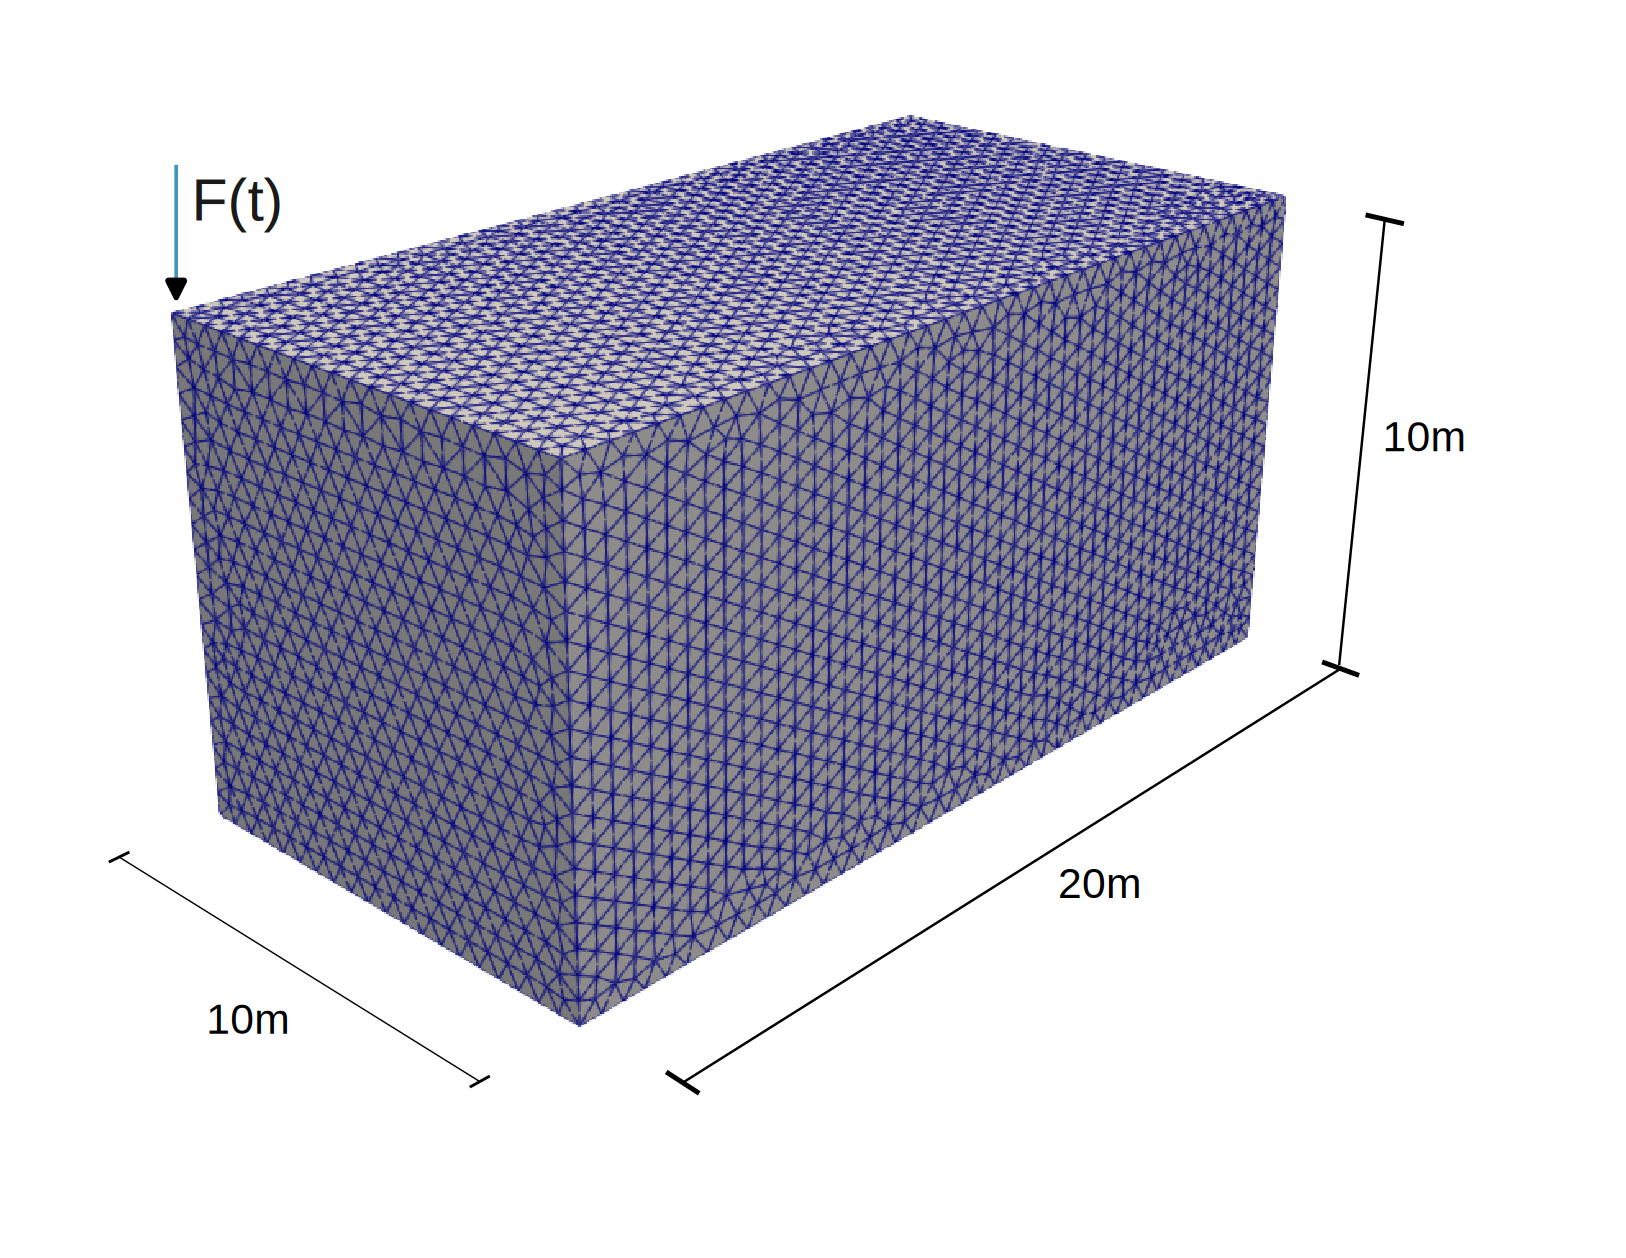
\includegraphics[width=0.75\textwidth]{strip_load_2D/mesh.png}
    \caption{Geometry, mesh and boundary conditions for the dynamic strip load problem.}
    \label{fig:strip2d_mesh}
\end{figure}

% ..............................................................................................
\subsection{Materials and Numerical Parameters}
% ..............................................................................................
The soil is modelled as an one-phase continuum with a linear elastic constitutive law, with the
following parameters:

\begin{itemize}[noitemsep,topsep=0pt,parsep=0pt,partopsep=0pt]
    \item Young's modulus: \qty{30}{\mega\pascal},
    \item Poisson ratio: 0.2,
    \item Density: \qty{2000}{\kilogram\per\meter\cubed}.
\end{itemize}

Material damping is included via Rayleigh damping, with parameters that provide a damping ratio of
\qty{0.5}{\percent} at \qty{1}{\hertz} and \qty{80}{\hertz}.


time integration uses a constant time step of \qty{0.001}{\second} within the \qty{0.20}{\second}
analysis window. The stiffness, mass and damping matrices are kept constant, and the system is solved
with a linear Newton--Raphson strategy combined with a direct LU factorisation, matching the solver
settings defined in the python test case.


% ----------------------------------------------------------------------------------------------
\section{Results}
% ----------------------------------------------------------------------------------------------

The validation focuses on the vertical velocity recorded at three nodes located along the loaded
surface at $(x,y) = (5,10)$, $(10,10)$ and $(15,10)$. Figure~\ref{fig:strip2d_results} compares the
STEM prediction against the stored Linux reference histories. The overlap of the two curves confirms
that the entire workflow---from geometry creation to Kratos execution and post-processing---remains
consistent for the 2D strip load scenario.

\begin{figure}[h]
    \centering
    \includegraphics[width=0.8\textwidth]{strip_load_2D/time_history.pdf}
    \caption{Vertical velocity time histories at the three monitored surface nodes for STEM and the
    Linux reference dataset.}
    \label{fig:strip2d_results}
\end{figure}
